\section{User Interface}
Considering the application is only a \acrshort{poc} there is almost no focus on the \acrlong{poc} nor on the \acrfull{ux}. To at least give a slight indication of what information needs to be displayed where, a \acrshort{ui} mock-up is created in Adobe Xd, Adobe Xd is a lightweight, rudimentary visual editor that enables designers to quickly develop and share interactive prototypes. A few example screens of the \acrshort{ui} prototype can be found below.
\begin{figure}[H]
\centering
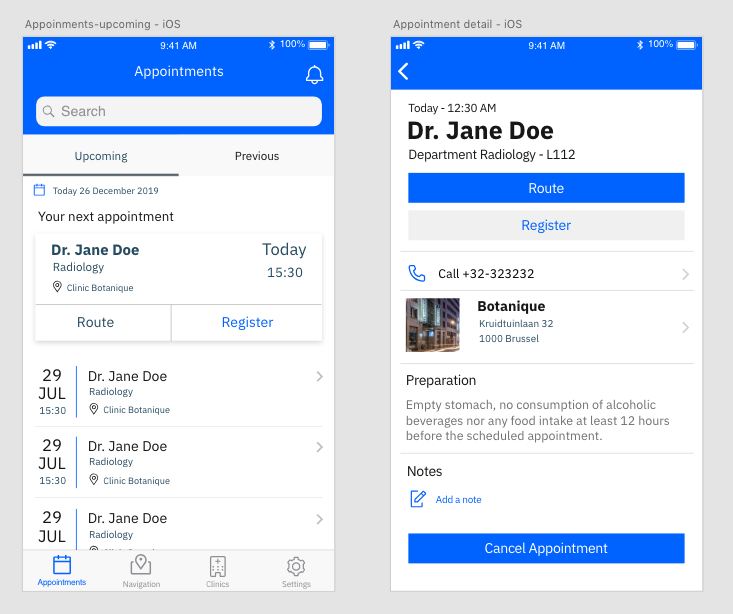
\includegraphics[scale=0.5]{appointments_screen_ios}
\caption{User interface of the appointments and detailed view for iOS}
\end{figure}
\begin{figure}[H]
\centering
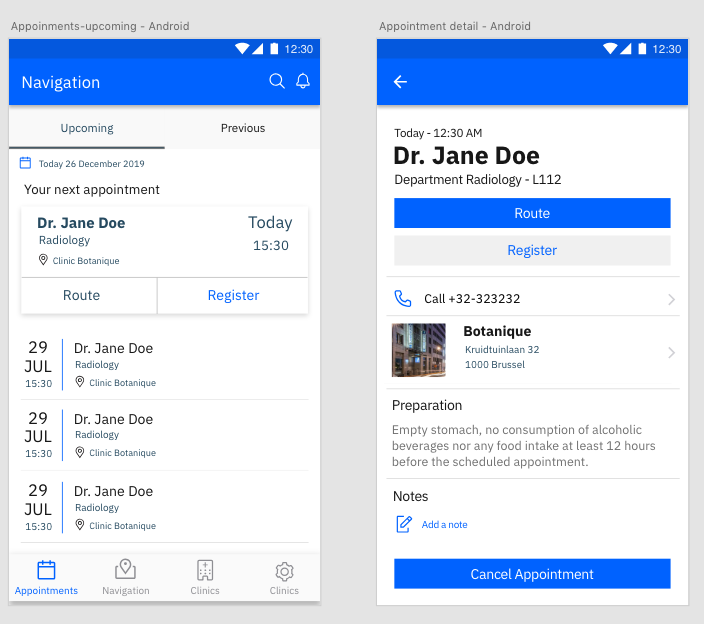
\includegraphics[scale=0.5]{appointments_screen_android}
\caption{User interface of the appointments and detailed view for Android}
\end{figure}
\begin{figure}[H]
\centering
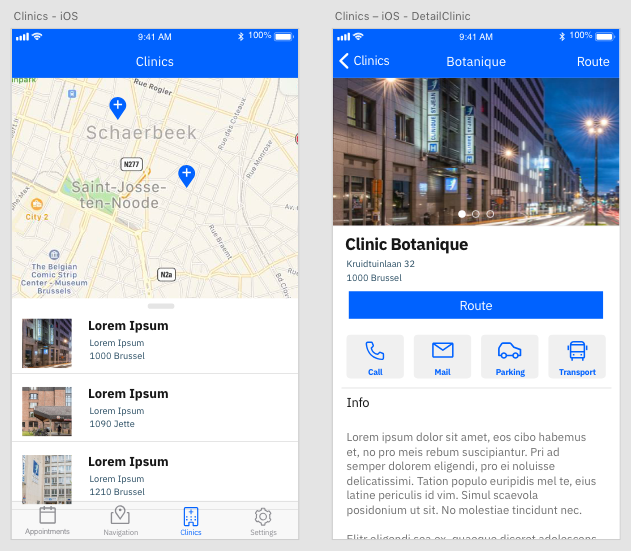
\includegraphics[scale=0.5]{clinics_screen_ios}
\caption{User interface of the hospital venues and detailed view for iOS}
\end{figure}
\begin{figure}[H]
\centering
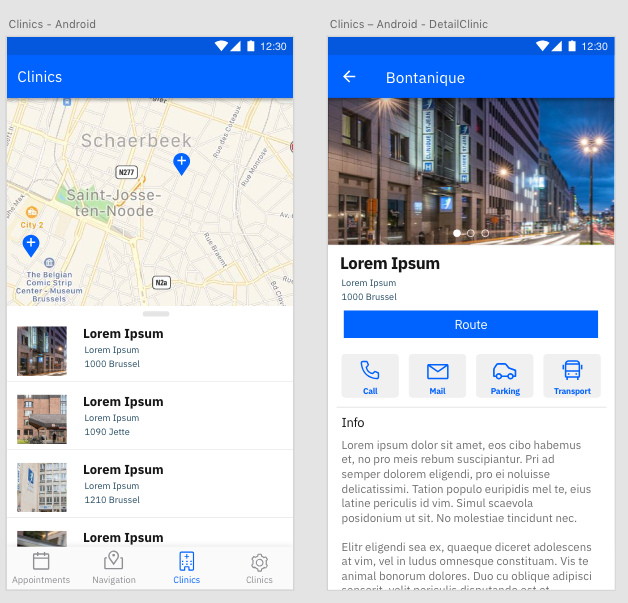
\includegraphics[scale=0.5]{clinics_screen_android}
\caption{User interface of the hospital venues and detailed view for Android}
\end{figure}
\section{General Data Protection Regulation}
\subsubsection{General Guidelines provided by the \acrfull{eu}}
\section{Database Communication}
\subsection{Testing API}
To aid in testing the database a test \acrshort{api} is programmed using a Node.js framework: Express. it is a very simple tool to create a web \acrshort{api} ready for consumption \cite{Express2019}. The testing \acrshort{api} is structured according to the entities specified in the \acrshort{uml} diagram with the corresponding relations. For this specific application there are a couple of endpoints exposed for requests:
\begin{itemize}
\item GET /appointments - this returns a JSON array containing test appointments;
\item GET /hospital - this returns information about the hospital such as address, contact details and venues;
\item GET /doctors - this fetches all the doctors present in the hospital records;
\item GET /departments - this returns all the departments available in the hospital and its venues;
\end{itemize}
\subsubsection{Faker}
Instead of using ad random numerical combinations or lorem ipsum texts, a library called Faker is used to generate different random values such are names, addresses, e-mail addresses and phone numbers. Faker is available for almost every general purpose language and is easy to use. It is always easier to work with representative data than it is to work with 'lorem ipsum' or '123456789' \cite{DanieleFaraglia2014}.
\subsection{IBM BlueMix API}

\section{Testing Application Programming Interface}
\section{Tools and frameworks used}
\section{MapWize}
MapWize is a service that digitalizes architectural plans and makes them interactive. MapWize offers an online environment in which you can easily create floor plans that can be used by the \acrshort{sdk}. In the online editor you can declare specific points of interest (PoIs) and routes from and to points. The creation of a digital map for testing purposes is out of scope for this thesis.
\subsection{MapWize SDK}
The team of developers at MapWize developed a completely open source \acrshort{sdk}, targeting the following platforms: iOS, Android, JS and \acrfull{pwa} \cite{MapWize.io2019a}. The one for Android has three versions: ready to use UI, bare-bones and an embedded WebView component.
\subsubsection{MapWize Barebone versus MapWize UI}
The bare-bones version of the \acrshort{sdk} comes as a plugin on top of the MapBox OpenGL library for Android. The Mapbox library handles the embedding of interactive vector assets into mobile applications \cite{Mabox2019}.

\section{Cisco Connectected Mobile Experiences integration}
The manner in which the position of a patient is retrieved is based on the nearest WiFi router of Cisco.
\subsection{Function of Cisco CMX}

\section{IndoorLocation Framework}
The IndoorLocation framework is one heavily used in conjunction with MapWize, it is a framework that allows developer to use geolocalization based on numerous indoor positioning technologies (IPS) such are: GPS, beacons, Wi-Fi, Li-Fi, Ultrasounds etc \cite{IndoorLocation.io2019}.



